%%%%%%%%%%%%%%%%%%%%%%%%%%%%%%%%%%%%%%%%%%%%%%%%%%%%%%%%%%%%%%%
%%%  notes
%%%%%%%%%%%%%%%%%%%%%%%%%%%%%%%%%%%%%%%%%%%%%%%%%%%%%%%%%%%%%%%

\documentclass[onecolumn,fleqn,notitlepage,secnumarabic]{revtex4}

% special 
\usepackage{ifthen}
\usepackage{ifpdf}
\usepackage{float}
\usepackage{color}

% fonts
\usepackage{latexsym}
\usepackage{amsmath} 
\usepackage{amssymb} 
\usepackage{bm}
\usepackage{wasysym}


\ifpdf
\usepackage{graphicx}
\usepackage{epstopdf}
\else
\usepackage{graphicx}
\usepackage{epsfig}
\fi

% packages added by jarondl
\usepackage{subfig}
\usepackage{verbatim} % for multiline comments
\usepackage{natbib} % change the bibliography style 
\usepackage{fancybox} % allows putting boxes with borders
\usepackage{cmap}  % for making pdf mathmode searchable
%\usepackage{sectsty}
\usepackage[pdftitle={Yaron de Leeuw's research proposal}]{hyperref}  % for hyperlinks in biblio. should be called last?

\graphicspath{{figures/},{PROG/figures/}}


%%%%%%%%%%%%%%%%%%%%%%%%%%%%%%%%%%%%%%%%%%%%%%%%%%%%%%%%%%%%%%%%

% NEW 
\newcommand{\abs}[1]{\left|#1\right|}
\newcommand{\varphiJ}{\bm{\varphi}}
\newcommand{\thetaJ}{\bm{\theta}}
%\renewcommand{\includegraphics}[2][0]{FIGURE}


% math symbols I
\newcommand{\sinc}{\mbox{sinc}}
\newcommand{\const}{\mbox{const}}
\newcommand{\trc}{\mbox{trace}}
\newcommand{\intt}{\int\!\!\!\!\int }
\newcommand{\ointt}{\int\!\!\!\!\int\!\!\!\!\!\circ\ }
\newcommand{\ar}{\mathsf r}
\newcommand{\im}{\mbox{Im}}
\newcommand{\re}{\mbox{Re}}

% math symbols II
\newcommand{\eexp}{\mbox{e}^}
\newcommand{\bra}{\left\langle}
\newcommand{\ket}{\right\rangle}

% Mass symbol
\newcommand{\mass}{\mathsf{m}} 
\newcommand{\rdisc}{\epsilon} 

% more math commands
\newcommand{\tbox}[1]{\mbox{\tiny #1}}
\newcommand{\bmsf}[1]{\bm{\mathsf{#1}}} 
\newcommand{\amatrix}[1]{\begin{matrix} #1 \end{matrix}} 
\newcommand{\pd}[2]{\frac{\partial #1}{\partial #2}}

% equations
\newcommand{\be}[1]{\begin{eqnarray}\ifthenelse{#1=-1}{\nonumber}{\ifthenelse{#1=0}{}{\label{e#1}}}}
\newcommand{\ee}{\end{eqnarray}} 

% arrangement
\newcommand{\hide}[1]{}
\newcommand{\drawline}{\begin{picture}(500,1)\line(1,0){500}\end{picture}}
\newcommand{\bitem}{$\bullet$ \ \ \ }
\newcommand{\Cn}[1]{\begin{center} #1 \end{center}}
\newcommand{\mpg}[2][1.0\hsize]{\begin{minipage}[b]{#1}{#2}\end{minipage}}
\newcommand{\mpgt}[2][1.0\hsize]{\begin{minipage}[t]{#1}{#2}\end{minipage}}



% extra math commands by jarondl
\newcommand{\inner}[2]{\left \langle #1 \middle| #2\right\rangle} % Inner product

%fminipage using fancybox package
\newenvironment{fminipage}%
  {\begin{Sbox}\begin{minipage}}%
  {\end{minipage}\end{Sbox}\fbox{\TheSbox}}


%%%%%%%%%%%%%%%%%%%%%%%%%%%%%%%%%%%%%%%%%%%%%%%%%%%%%%%%%%%%%%%%%%%%%%%%%%%

% Page setup
\setlength{\parindent}{0cm} 
\setlength{\parskip}{0.3cm} 

%%% Sections. The original revtex goes like this:
%\def\section{%
%  \@startsection
%    {section}%
%    {1}%
%    {\z@}%
%    {0.8cm \@plus1ex \@minus .2ex}%
%    {0.5cm}%
%    {\normalfont\small\bfseries}%
%}%
%\def\subsection{%
%  \@startsection
%    {subsection}%
%    {2}%
%    {\z@}%
%    {.8cm \@plus1ex \@minus .2ex}%
%    {.5cm}%
%    {\normalfont\small\bfseries}%
%}%
%%%%%%% And our version goes like this:
\makeatletter
\def\section{%
  \@startsection
    {section}%
    {1}%
    {\z@}%
    {0.8cm \@plus1ex \@minus .2ex}%
    {0.5cm}%
    {\Large\bf $=\!=\!=\!=\!=\!=\;$}%
}%
\def\subsection{%
  \@startsection
    {subsection}%
    {2}%
    {\z@}%
    {.8cm \@plus1ex \@minus .2ex}%
    {.5cm}%
    {\normalfont\small\bfseries$=\!=\!=\!=\;$}%
}%
%%%%%%%%%%  Here we deal with capitalization. The original revtex first, and then our version.
%\def\@hangfrom@section#1#2#3{\@hangfrom{#1#2}\MakeTextUppercase{#3}}%
%\def\@hangfroms@section#1#2{#1\MakeTextUppercase{#2}}%
\def\@hangfrom@section#1#2#3{\@hangfrom{#1#2}{#3}}%
\def\@hangfroms@section#1#2{#1{#2}}%
\makeatother


%%%%%%%%%%%%%%%%%%%%%%%%%%%%%%%%%%%%%%%%%%%%%%%%%%%%%%%%%%%%%
%%%%%%%%%%%%%%%%%%%%%%%%%%%%%%%%%%%%%%%%%%%%%%%%%%%%%%%%%%%%%
\begin{document}

\title{Diffusion properties of mesoscopic systems}

\author{Yaron de Leeuw \\ Adviser: Professor Doron Cohen}
\affiliation{Physics Department, Ben Gurion University of the Negev}
\date{\today}
\maketitle


%%%%%%%%%%%%%%%%%%%%%%%%%%%%%%%%%%%%%%%%%%%%%%%%%%%%%%%%%%%%%%%%%%%%%%%%%%%%%%%%%%%%%%%%%%%%
%%%%%%%%%%%%%%%%%%%%%%%%%%%%%%%%%%%%%%%%%%%%%%%%%%%%%%%%%%%%%%%%%%%%%%%%%%%%%%%%%%%%%%%%%%%
%%%%%%%%%%%%%%%%%%%%%%
\section{Introduction}

%%%%%%%%%%%
\subsection{Defining site occupation probabilities and transition rates}
First let us define the model. The model consists of sites which a particle may occupy. At each point in time, and for every site, there is a probability to find the particle in this particular site, which is called \emph{occupation probability}. We define the \emph{transition rates} as the rate in which those probabilites move from one site to another. A $1d$ system can also be called a Markovian chain. Higher dimensional systems are types of networks, or \emph{graphs}, where \emph{Graph Theory} has some relevance.

%%%%%%%%%%%
\subsection{Rate equation}
We use $P_n$ to denote the $n$'th site occupation probability, and $W_{nm}$ for the transition rate between two sites $n$ and $m$. The time evolution of $P_n$ may be written as:
\begin{align}
\frac{dP_n(t)}{dt} = \sum_m W_{nm}P_m(t)
\end{align}
Because of probability conservation, we want to have $\sum_m W_{nm} = 0 \  \forall m$ , which we can achieve by setting $W_{nn} = -\sum_{m\ne n} W_{nm} $, meaning that for each site the sum of incoming transition rates negates the outgoing transitions.

In a vector form, we have:
\begin{align} \boldsymbol{ \dot P } = \boldsymbol{W} \boldsymbol{P} \end{align}
The vector $\boldsymbol{P}$ has positive values and sums up to one. The matrix $\boldsymbol{W}$ is symmetric (at the moment, see section \ref{sec:vrh}), except for the main diagonal, which has values that ensure that each row's sum is zero.

%%%%%%%%%%%
\subsection{Deciding the values for the the transition rates}
Most of the systems we will work with can be defined unambiguously by defining their transition rates. We can map certain physical, geometrical or topological charecteristics of systems to their transition rate matrices. One of our main interests are transition rates that depened on the distance betweeen scattered points, in either $1d$, $2d$, or any other dimension. Specifically, the case of $W_{nm}= e^{-r_{nm}/ \xi}$, which was studied by \citet{Amir:2010:PRL}, will be researched.

%%%%%%%%%%%%%%%%%%%%%%%%%%%%%%%%%%%%%
\section{TEMP TITLE: What we seek and for which models}

%%%%%%%%%%%
\subsection{Survival probability - $\mathcal{P}(t)$} 
The survival probability is the probability to remain in the starting site. If the initial condition was $P_0(0)=1$, $P_i(0)=0 \textrm{  for  } i\neq 0$, then $\mathcal{P}(t)= P_0(t)$. The survival probability is related to the localization properties of the system.

%%%%%%%%%%%
\subsection{Transport / Conductance / Spreading}
All these terms refer to quantities that measure at which rate does a particle move in the system. Spreading usually means the Root-Mean-Square of the particle from its initial position, while Conductance is the rate at which particles pass the system from one end to the other.

%%%%%%%%%%%
\subsection{$1d$, $2d$, quasi-$1d$}

%%%%%%%%%%%%%%%%%%%%%%%%%%%%%%%%%%%%%
\section{Block renormalization group}
A useful method to find the conductance is block renormalization. For $1d$ this is rather straight forward. In each step two adjacent bonds are treated as one renormalized bond. This is repeated until we have one effective bond, instead of the entire system. (See figure \ref{fig:renorm_group}). 
\begin{figure}
    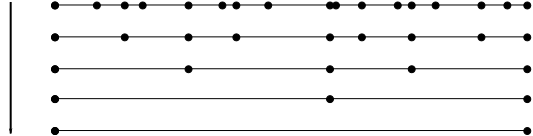
\includegraphics[clip]{rp_renorm_group}
    \caption{Block renormalization in $1d$. The dots represent sites, while the lines represent bonds.}
    \label{fig:renorm_group}
\end{figure}

For $2d$ or higher, we will need another mechanism, because cutting the system to blocks is not as trivial. In $1d$, two adjacent bonds have two connections to the rest of the system, and thus the replacement procedure is trivial. In $2d$, each site has many bonds, so to remove a site many bonds need to be renormalized which is rather difficult. An optional solution is to treat the network as continuous, and then slice it geometrically.


\section{Adding site-energy to the game} \label{sec:vrh}
If the sites have different potentials, then the probability to remain in a site is modified by Boltzmann's factor. The VRH - \emph{Variable Range Hopping} method compensates for this effect by altering the transition rates accordingly. In VRH, the transition rate matrix stays symmetric, meaning that the transition rate from site $A$ to site $B$ equals the rate from $B$ to $A$. However, we know that transition from a higher potential site to a lower potential one is more probable than the reverse, by Boltzmann's factor. Therefore, we know that the matrix cannot be symmetric, and Boltzmann's factor should be added. It is of great interest to us wheter this change is significant, and how does it affect our current knowledge about survival and conductance.


%\bibliographystyle{plainnat}
\bibliography{jarondl}
\end{document}
